%\begin{multicols}{2}

\cappar
\
\begin{center}
``Los rumores son como la crecida de un río, no se pueden frenar.''
\end{center}

Para este número os tenemos preparado un problema que muestra porque los rumores o chismes se mueven tan rápidos. También os dejamos un nuevo reto ajedrecístico y os hablamos de una modalidad de ajedrez que permite enseñar a niños y mayores de una manera mucho más colorida que la usual.

 ¡Esperamos que disfruten! 

\section*{El chisme}

A las 10 de la mañana llegó un caballero extranjero llegó a una ciudad de 50.000 habitantes. Este caballero tenía conocimiento de un mensaje bastante importante de interés general. Cuando llegó al hotel donde se iba a hospedar el caballero comunicó ese mensaje a 3 personas de esa ciudad. Digamos que esto ocurrió en un cuarto de hora. Esto quiere decir que a las 10 y cuarto de la mañana 4 personas eran conocedoras del mensaje: 3 habitantes de la ciudad y el caballero extranjero. Conocida la noticia cada uno de los 3 habitantes se apresuró a contarle la noticia a 3 personas más. ¿A qué hora ya podriamos asegurar que el mensaje era conocido por toda la ciudad? 

\section*{Ajedrez}

Un reto y una novedad.

\subsection*{Belleza al ganar}

Observa la partida en la Figura \ref{partida}. La situación de las blancas parece prometedora, por su buena coordinación, pero también muy apurada, porque si se limitan a defender el caballo, con Ab4, el rey negro mejoraría, con Rc7; y si mueven el jamelgo, la dama negra se activa y da jaques. ¿Hay alguna otra solución? Pero, ¿se te ocurre alguna otra solucion? ¿Una solución más bonita?. Mándanos tu respuesta al siguiente email: \url{mpelaezmath@gmail.com}.
\begin{figure}[!ht]
\centering 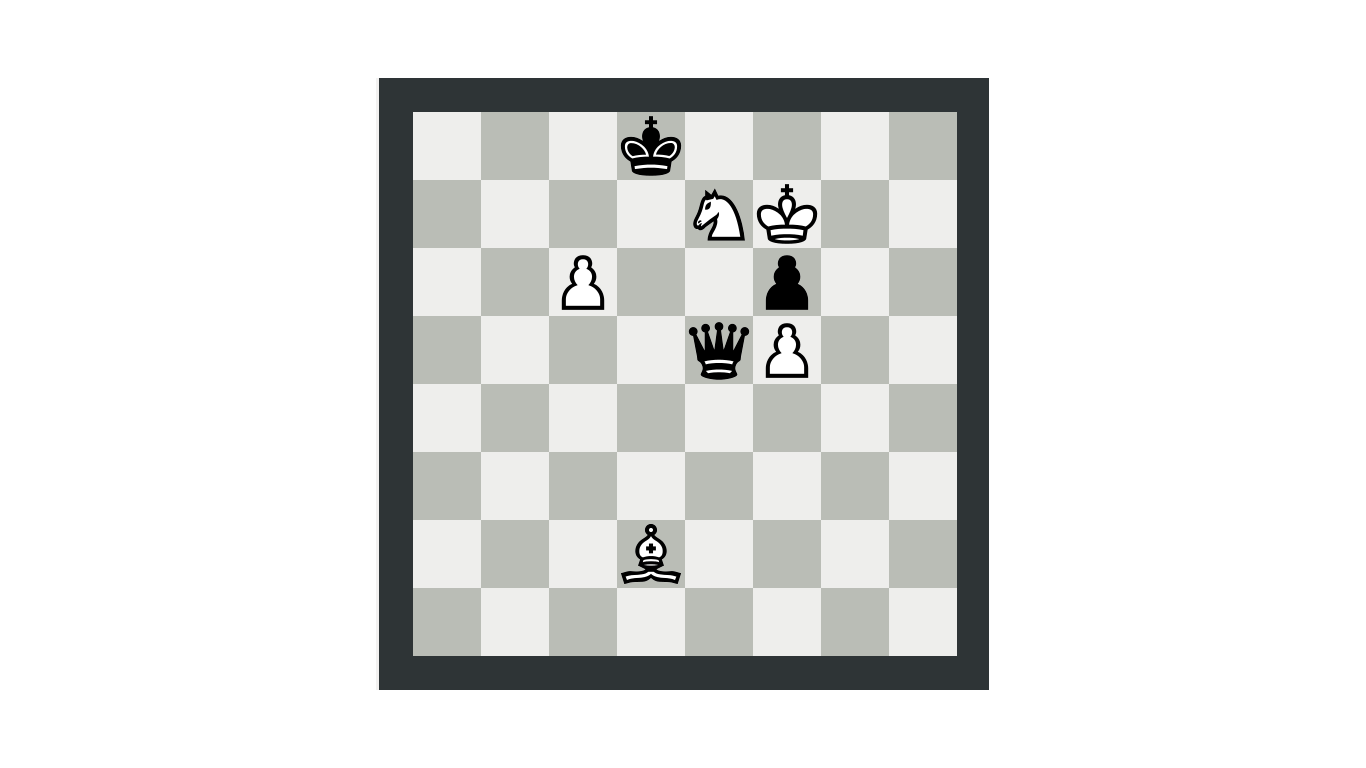
\includegraphics[scale=0.2]{partida2.png}
\caption{Reto ajedrecístico}\label{partida}
\end{figure}

% respuesta está en http://www.elpais.com/misc/ajedrez/5abril14.htm
%Te ofrecemos un reto ajedrecístico. En esta famosa partida, que te desvelaremos en el siguiente número, 
%las blancas juegan y ganan. ¿Podrías encontrar la espectacular jugada ganadora?
% http://www.tabladeflandes.com/internacionales_2013/pgn-Carlsen-Anand-2013.php?partida=9&cor1=Negras&cor2=Blancas&rdo1=1&rdo2=0
% Campeonato del Mundo Ajedrez 2013- Chennai. India. 7 - 28	Noviembre 2013 
% MAGNUS CARLSEN CAMPEÓN DEL MUNDO
% Ajedrez para niños: http://chesslive.com/blog/2014/03/13/en-directo-candidatos-de-ajedrez-2014/
% Canal argentino: http://www.tabladeflandes.com/nuestro_circulo.php
%\newgame
%\mainline{1. d4 Nf6 2. c4 e6 3. Nc3 Bb4 4. f3 d5 5. a3 Bxc3+ 6. bxc3 c5 7. cxd5 exd5 8. e3 c4 9. Ne2 Nc6 10. g4 O-O 11. Bg2 Na5 12. O-O Nb3 13. Ra2 b5 14. Ng3 a5 15. g5 Ne8 16. e4 Nxc1 17. Qxc1 Ra6 18. e5 Nc7 19. f4 b4 20. axb4 axb4 21. Rxa6 Nxa6 22. f5 b3 23. Qf4 Nc7 24. f6 g6 25. Qh4 Ne8 26. Qh6 b2 27. Rf4 b1=Q+ 28. Nf1 Qe1}



\subsection*{Una nueva modalidad de jugar ajedrez: con colores}
El Ajedrez de Colores es un educativo, creativo y divertido juego basado en las reglas del ajedrez. Las casillas negras del tablero pueden ser de distintos colores, cada uno de estos colores indica como mover en el juego. Todas las piezas son peones y pueden customizarse, de inicio están sobre casillas blancas y mueven como un Rey de Ajedrez, pero al moverlos a cada una de las casillas de color, se irán convirtiéndose en Dama, Rey, Torre, Alfil o Caballo, según el color de la casilla en la que se sitúen y moverán exactamente igual que en el Ajedrez. El objetivo del juego es convencer (dar jaque mate)  al Peón que hayas elegido como Líder.

El ajedrez de colores está creado con la finalidad de desarrollar habilidades que se trabajan con el ajedrez clásico con el añadido de que la curva de aprendizaje de este juego es más rápida y esto puede atraer a nuevos jugares. 

El pionero de esta modalidad ajedrecista es el español Jose María Cortés. Puede tener más información al respecto en la siguiente web \url{http://www.ajedrezdecolores.es/} en la cual se te permite jugar online y aprender todas las opciones que posee (véase Figura  \ref{colores}).

\begin{figure}[!ht]
\centering 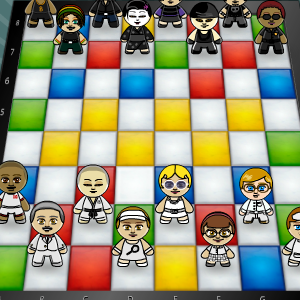
\includegraphics[scale=0.4]{colores.png}
\caption{Ajedrez de colores}\label{colores}
\end{figure}

\section*{\textcolor{redsol}{Soluciones del número anterior}}
\subsection*{La balanza}
La respuesta del desafío de la balanza la encontramos tratando de conseguir todos los posibles pesos entre 1 y 40 kilos. Es
decir, buscar una forma de pesar, entre los dos platillos y las cuatro pesas que tenemos, todos los números (en kilos) entre 1 y 40.

Empezamos:
\begin{dinglist}{234}
\item Para el número 1, no hay problemas. Basta con poner sobre uno de los platillos la pesa con el número 1.
\item ¿Cómo hacer con el 2? Está claro que no hay pesa que ‘pese’
exactamente dos kilos. Sin embargo, si yo pongo de un lado
la de 3 kilos y del otro lado la de 1 kilo, está claro que la diferencia entre los dos platillos es lo que quiero pesar: 2 kilos.
\item Tres kilos: usando sólo la pesa de 3 kilos.
\item Cuatro kilos: ponemos en un platillo las pesas de 1 kilo y de 3 kilos.
\item Cinco kilos: ponemos en un platillo la pesa de 9 kilos y en otro platillo las pesas de 1 y 3 kilos, la diferencia nos da cinco kilos.
\item \dots
\end{dinglist}
Y de este modo vamos combinando hacia un plato y otro y obtenemos todos los pesos de 1 a 40, mostramos todos los resultados a continuación:
\begin{multicols}{3}
\begin{itemize}
\item $1=1-0$
\item $2=3-1$
\item $3=3-0$
\item $4=(3+1)-0$
\item $5=9-(3+1)$
\item $6=9-3$
\item $7=(9+1)-3$
\item $8=9-1$
\item $9=9-0$
\item $10=(9+1)-0$
\item $11=(9+3)-1$
\item $12=(9+3)-0$
\item $13=(9+3+1)-0$
\item $14=27-(9+3+1)$
\item $15=27-(9+3)$
\item $16=(27+1)-(9+3)$
\item $17=27-(9+1)$
\item $18=27-9$
\item $19=(27+1)-9$
\item $20=(27+3)-(9+1)$
\item $21=(27+3)-9$
\item $22=(27+3+1)-9$
\item $23=27-(3+1)$
\item $24=27-3$
\item $25=(27+1)-3$
\item $26=27-1$
\item $27=27-0$
\item $28=(27+1)-0$
\item $29=(27+3)-1$
\item $30=(27+3)-0$
\item $31=(27+3+1)-0$
\item $32=(27+9)-(3+1)$
\item $33=(27+9)-3$
\item $34=(27+9+1)-3$
\item $35=(27+9)-1$
\item $36=(27+9)-0$
\item $37=(27+9+1)-0$
\item $38=(27+9+3)-1$
\item $39=(27+9+3)-0$
\item $40=(27+9+3+1)-0$
\end{itemize}
\end{multicols}
%\end{multicols}

\subsection{Ajedrez}
La partida que se presentó en la edición pasada es una partida del año 1941 disputada entre el ruso Alekhine contra Supico. Alekhine fue un jugador excelente de ajedrez que murió siendo el campeón mundial de ajedrez. Y la posición que lleva a las blancas ser ganadoras es la dama a g6. De esta forma las negras deben deponer sus armas y las blancas ganan. ¿Lo descubriste?
\newgame
\hidemoves{1. e4 e5 2. d4 exd4 3. c3 dxc3 4. Nxc3 Bb4 5. Bc4 Qe7 6. Ne2 Nf6 7. O-O O-O 8. Bg5 Qe5 9. Bxf6 Qxf6 10. Nd5 Qd6 11. e5 Qc5 12. Rc1 Qa5 13. a3 Bxa3 14. bxa3 c6 15. Ne7 Kh8 16. Qd6 Qd8 17. Nd4 b6 18. Rc3 c5 19. Ndf5 Ba6}
% 20. Qg6}
\tinyboard
\begin{center}
%\printarrow{e2}{e4} 
\showboard 
\hidemoves{20. Qg6} $\Rightarrow$
\showboard
\end{center}
\newpage


%%% Local Variables:
%%% mode: latex
%%% TeX-master: "jugando"
%%% End:



